\documentclass{scrartcl}			% defines the kind of document you want to produce

% Include different packages:
\usepackage[utf8]{inputenc}
\usepackage[T1]{fontenc}
\usepackage{lmodern}
\usepackage[english]{babel}
\usepackage{amsmath}
\usepackage{float}
\usepackage{graphicx}           	% include graphics
\usepackage{caption}
\usepackage{subcaption}
\usepackage{hyperref}

\title{Neuroprothetik Exercise 1}
\author{Aleksandra Teska}
\date{26. April 2018}


\begin{document} 					% Document begins here

\maketitle

\section{Generate a signal}		% start a new section
The goal of this exercise was creating a Python function that given following inputs:

a) An array of frequencies (in Hz)

b) An array of amplitudes

c) The signal duration (in seconds)

d) The sample rate (in Hz)

, which returns signal given by equation:
\begin{align}
f(t) = A_0 + \sum_{i=1}^{n} A_i sin(2\pi F_i\cdot t)
\end{align}			
 
where $A_{i}$ is the amplitude of the frequency component $F_{i}$  and  $A_{0}$  is the signal offset

\subsection{Plot the signal}		% start a new subsection
The implemented function was used to generate a one second long signal, consisting of the frequency components 100 Hz, 600 Hz and 9 kHz with the amplitudes 1, 1.5 and 2, an offset of 3 at a sampling rate of 100 kHz.
The first 100 ms of the signal were plotted in Figure \ref{subsec_fig}




\section{Calculate the spectrum}
The goal of the second exercise was calculating the single sided amplitude spectrum (positive half) of the signal, with the use of Fast Fourier Transformation. For this exercise Python function \textit{numpy.fft.fft(signal)} was used. Function works as follows:
\begin{itemize}
	\item Calculate FFT with numpy function
	\item Divide the returned values by the number of input samples 
	\item Add up positive and negative frequency bins
	\item Return single sided amplitude spectrum of a given signal
\end{itemize}

\subsection{Plot the Spectrum}
The spectrum of the same signal as in exercise one was generated, for sampling rates of: 100kHz, 20 kHz and 10 kHz  Results plotted in Figure \ref{fig:figure}




\subsection{Results}
With the use of first sampling rate value of 100 kHz we can see an accurate representation of the amplitudes of generated signals. In the middle single sided amplitude spectrum, calculated with the sampling rate of 20 kHz, the amplitude of 9kHz frequency component of the signal is decreased. It might be a result of numerical errors coming from numpy FFT() function.\\

In case of the bottom amplitude spectrum, we can see the results of using a too low sampling rate value. According to the \textit{Nyquist–Shannon sampling theorem} the sampling frequency should be at least two times higher then the recorded signal. According to theory and in case of the generated signal, sampling rate should be equal to at least 18 kHz. On the plotted spectrum we can notice an aliasing effect, due to which the last pick of 9kHz frequency can be now seen at the point of 1 kHz.\\

Signal can be recorded with the sampling rates of 100 kHz. To record such a signal with the given sample rates lower then 18 kHz (in example 10 kHz), we would have to use anti-aliasing filter (low pass filter), that would attenuate the higher frequencies (greater than the Nyquist frequency), it prevents the aliasing components from being sampled.


\begin{figure*}[hbpt!]					%start figure-environment
	\centering
	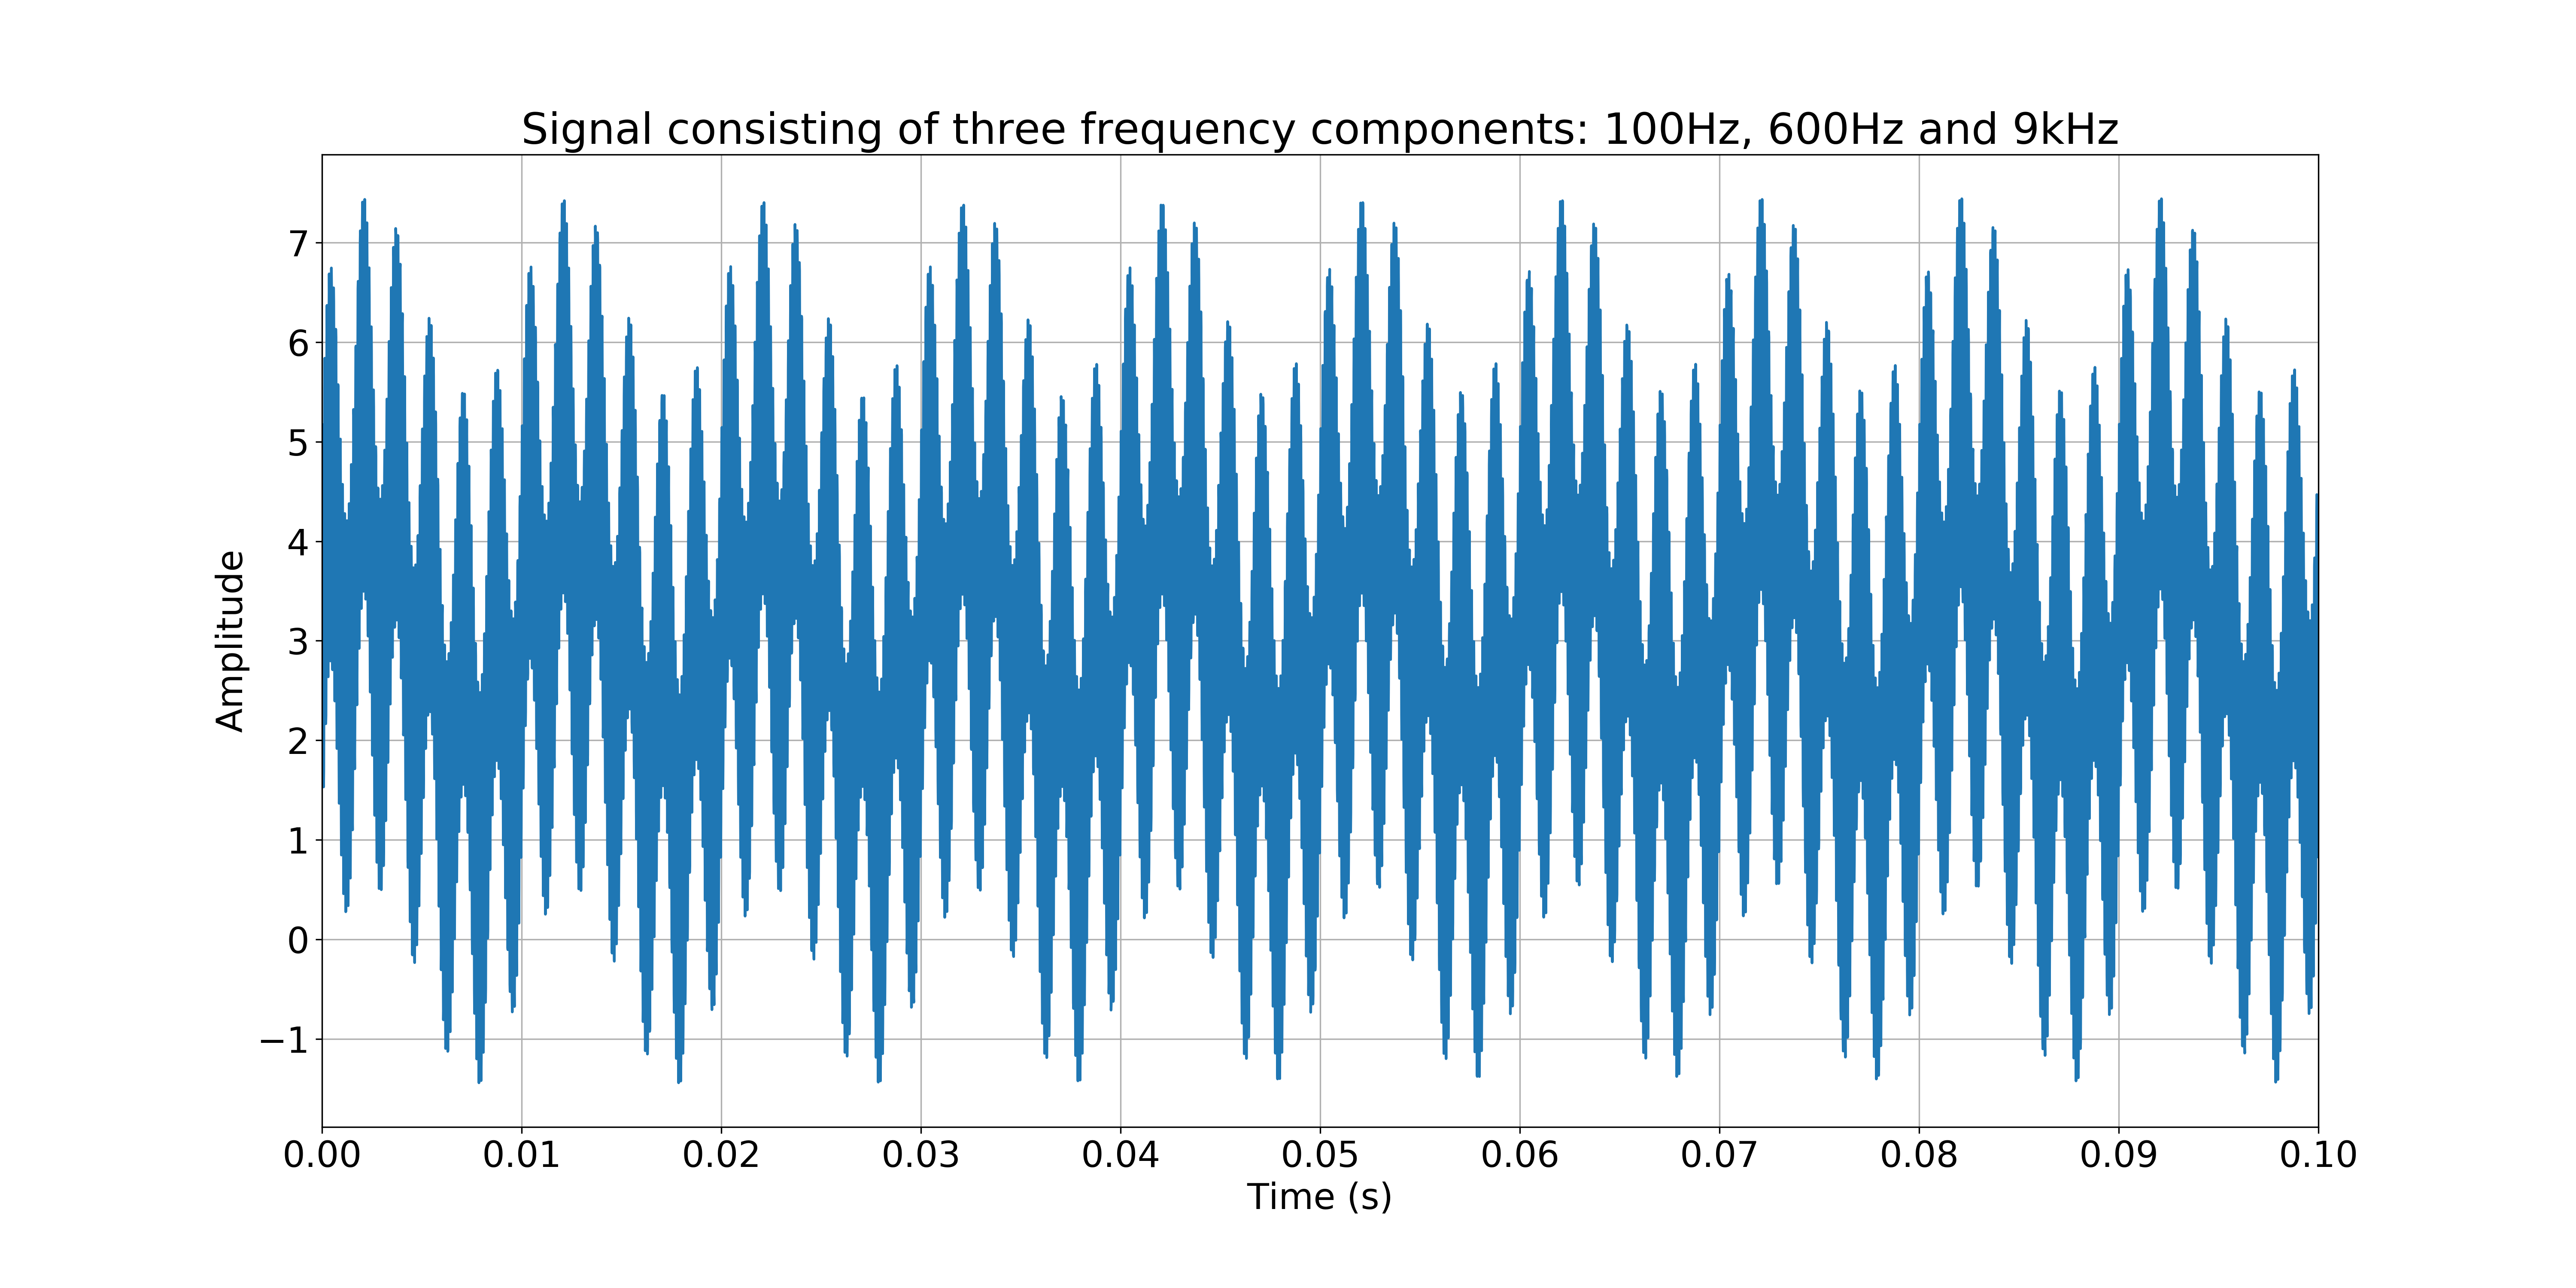
\includegraphics[scale=0.3]{1.png}
	\captionsetup{width=\linewidth}  %choose the with of the caption
	\caption{Solution to 1.1. The first 100 ms of the created signal which was sampled with a sampling-frequency of 100 kHz.}
	\label{subsec_fig} %choose a label, see subsection references
\end{figure*}


\begin{figure*}[hbpt!]					%start figure-environment
	\centering
	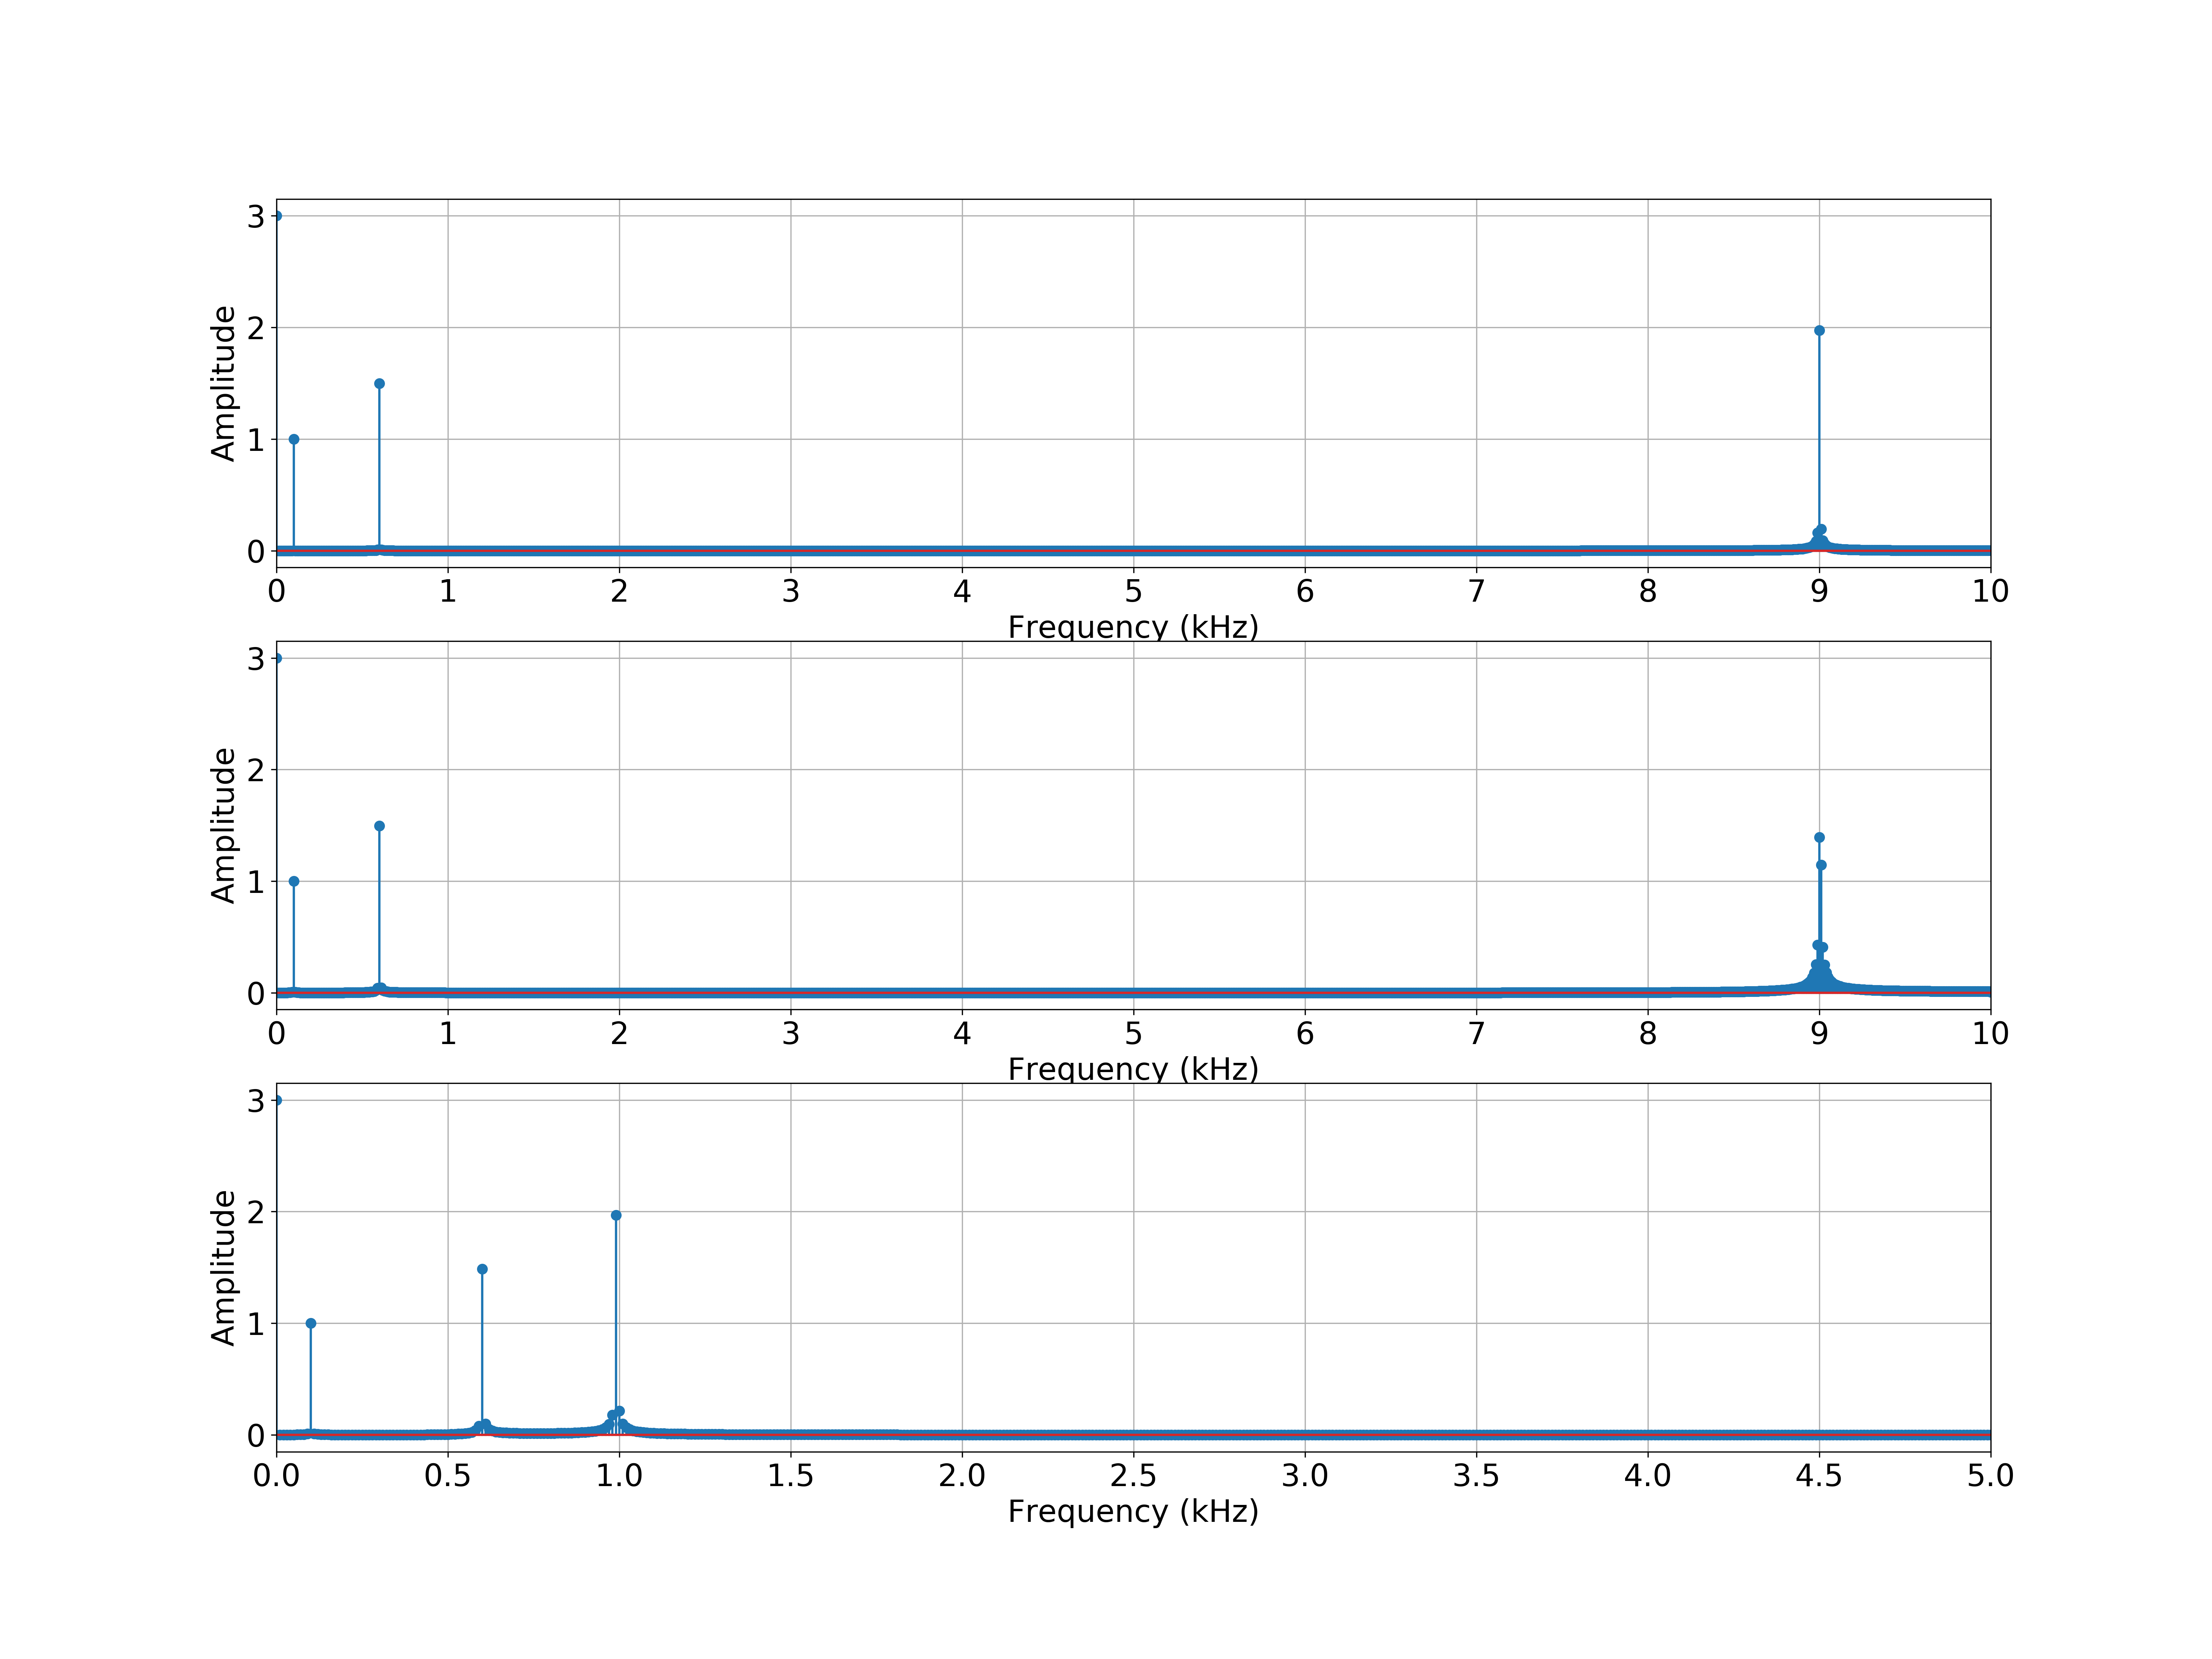
\includegraphics[scale=0.3]{2.png}
	\captionsetup{width=\linewidth}  %choose the with of the caption
	\caption{Solution to 2.1. Different FFTs of the signal shown in figure 1. Top: sampling frequency is
		100 kHz, only frequencies up to 10 kHz are shown. Middle: sampling frequency is	20 kHz. Bottom: sampling frequency is 10 kHz}
	\label{fig:figure} %choose a label, see subsection references
\end{figure*}

\end{document}
